\documentclass[11pt,a4paper]{article}

% ---------- Packages ----------
\usepackage[utf8]{inputenc}
\usepackage[T1]{fontenc}
\usepackage[english]{babel}
\usepackage{amsmath,amssymb,bm}
\usepackage{graphicx}
\usepackage{subcaption}
\usepackage{booktabs}
\usepackage{siunitx}
\usepackage{geometry}
\usepackage{hyperref}
\usepackage{float}
\usepackage{caption}
\usepackage{microtype}
\usepackage{setspace}

\geometry{margin=2.5cm}
\onehalfspacing

\hypersetup{
    colorlinks=true,
    linkcolor=black,
    citecolor=blue,
    urlcolor=blue
}

\graphicspath{{plots/}}

\title{\textbf{Coarsening and Arrest in Colloidal Gels:}\\
Modelling via Brownian Dynamics}
\author{B\'er\'enice Derai --- 66034}
\date{5 June 2026}

\begin{document}

\maketitle

\begin{abstract}
This project explores the dynamics of colloidal gels, focusing on the processes of coarsening and arrest. A minimal model of attractive Brownian particles is constructed and their dynamics are simulated using an Euler--Maruyama scheme with a Lennard--Jones pair potential. The growth of the structure factor $S(k,t)$ is analysed by comparing two regimes: a strongly attractive system, $\varepsilon = 5 k_B T$, exhibiting incipient kinetic arrest, and a weakly attractive liquid reference, $\varepsilon = 1.5 k_B T$, that undergoes continuous coarsening.

An ageing study is additionally performed: the mean-squared displacement (MSD) is computed for multiple waiting times $t_w$. In a fully arrested gel, one expects waiting-time-dependent dynamics, whereas an ergodic liquid should show an approximate collapse of MSD curves for different $t_w$. Several numerical challenges, including integrator instability, inadequate simulation time, and an unphysical reference state, were identified and corrected iteratively. The theoretical framework draws on the works of Doi for statistical mechanics and colloidal diffusion, and on the literature on ageing and non-equilibrium states.
\end{abstract}

\tableofcontents
\newpage

% ============================================================
\section{Introduction}

Colloidal suspensions are systems composed of particles with typical sizes between $1\,\mathrm{nm}$ and $1\,\mu\mathrm{m}$ dispersed in a solvent.  When sufficiently strong attractive interactions are induced between colloidal particles, for example by the addition of salt in a charged suspension, by polymer depletion, or by unscreened van der Waals interactions, the system may undergo phase separation towards a dense state. However, the intrinsically slow dynamics of massive colloidal particles can trap the system in a non-equilibrium state before phase separation is complete. This phenomenon is known as gelation by arrested phase separation.

The goal of this work is to construct a minimal model of attractive Brownian particles, to simulate its dynamics using an Euler--Maruyama scheme, and to analyse the growth of the structure factor $S(k,t)$ in the presence and absence of gelation. An ageing study based on the mean-squared displacement is also carried out in order to probe the non-ergodic character of the arrested gel.

The report is organised as follows. First, the theoretical background of Brownian motion, colloidal diffusion, and attractive interactions is introduced. The mechanism of phase separation and gelation by kinetic arrest is then discussed. The structure factor is presented as the central observable used to characterise coarsening and dynamic scaling. Finally, the numerical implementation and simulation results are analysed, with a particular focus on the comparison between a gel regime and a weakly attractive liquid reference.

% ============================================================
\section{Brownian Motion and Colloidal Diffusion}

\subsection{The Langevin Equation}

Following Doi, the motion of a colloidal particle suspended in a solvent can be described by separating the force exerted by the fluid into two contributions: a deterministic viscous friction force and a stochastic random force arising from microscopic collisions with solvent molecules.

The equation of motion is the Langevin equation
\begin{equation}
    m\ddot{\mathbf r}
    =
    -\zeta \dot{\mathbf r}
    -\nabla U
    +
    \mathbf F_r(t),
    \label{eq:langevin}
\end{equation}
where $-\zeta \dot{\mathbf r}$ is the viscous friction force, $U(\mathbf r)$ is the interaction potential, and $\mathbf F_r(t)$ is the stochastic random force.

For a spherical colloid of radius $a$ immersed in a solvent of viscosity $\eta$, the Stokes friction coefficient is
\begin{equation}
    \zeta = 6\pi\eta a.
\end{equation}
The random force satisfies
\begin{equation}
    \langle \mathbf F_r(t)\rangle = 0,
\end{equation}
and obeys the fluctuation--dissipation theorem
\begin{equation}
    \left\langle F_{r,\mu}(t)F_{r,\nu}(t')\right\rangle
    =
    2\zeta k_B T\,\delta_{\mu\nu}\delta(t-t').
    \label{eq:fdt}
\end{equation}
This relation ensures that thermal fluctuations compensate viscous dissipation and maintain thermal equilibrium at temperature $T$.

\subsection{Overdamped Limit: Brownian Dynamics}

For colloidal particles, the inertial relaxation time
\begin{equation}
    \tau_m = \frac{m}{\zeta}
\end{equation}
is typically of order $10^{-8}\,\mathrm{s}$, whereas the diffusive timescale
\begin{equation}
    \tau_D = \frac{a^2}{D}
\end{equation}
is of order $10^{-3}\,\mathrm{s}$. Since $\tau_m \ll \tau_D$, inertia relaxes much faster than diffusion and the inertial term can be neglected. The Langevin equation therefore reduces to
\begin{equation}
    \dot{\mathbf r}
    =
    -\frac{D}{k_B T}\nabla U
    +
    \frac{1}{\zeta}\mathbf F_r(t),
    \label{eq:bd}
\end{equation}
where the Einstein relation
\begin{equation}
    D = \frac{k_B T}{\zeta}
\end{equation}
has been used.

This overdamped description forms the basis of Brownian Dynamics simulations.

% ============================================================
\section{Colloidal Interactions}

\subsection{Pair Potentials Between Colloids}

Two particles of radius $a$ cannot overlap. This excluded-volume constraint is represented by a hard-core interaction. In addition to repulsion, colloidal particles interact through attractive forces. Quantum fluctuations of electronic dipoles generate long-range van der Waals attractions between dielectric materials.

For charged particles dispersed in an electrolyte, the DLVO theory describes the competition between electrostatic repulsion and van der Waals attraction. Increasing the salt concentration screens electrostatic interactions, lowers the repulsive barrier, and can render the effective interaction attractive at short distances. 

\subsection{Choice of Potential for Simulations}

The simulations performed in this work use a truncated and shifted Lennard--Jones potential,
\begin{equation}
    U_{\mathrm{LJ}}(r)
    =
    4\varepsilon
    \left[
    \left(\frac{\sigma}{r}\right)^{12}
    -
    \left(\frac{\sigma}{r}\right)^6
    \right]
    -
    U_{\mathrm{LJ}}(r_{\mathrm{cut}}),
    \label{eq:lj}
\end{equation}
where the shift $U_{\mathrm{LJ}}(r_{\mathrm{cut}})$ ensures continuity of the potential at the cutoff. The cutoff is set to $r_{\mathrm{cut}} = 2.5\sigma$ for both regimes, which retains the attractive well in its entirety while keeping the computational cost of the force loop tractable; beyond $2.5\sigma$ the LJ interaction is less than $0.02\,\varepsilon$ and can be safely neglected.

While the DLVO theory provides the physical mechanism for attraction — electrostatic screening by added salt reduces the repulsive barrier, leaving the van der Waals attraction dominant at short range — it yields a multi-parameter potential difficult to parametrise in a minimal simulation model. The Lennard--Jones potential is used here as an effective pair potential capturing the essential physics in a single analytically tractable form: the $r^{-12}$ term mimics hard-core exclusion, and the $-r^{-6}$ term captures the net short-range attraction once the electrostatic barrier is screened. Compared to the originally planned Morse potential, the LJ form requires only one energy parameter $\varepsilon$ (the Morse potential additionally requires an equilibrium distance $r_{\mathrm{eq}}$ and a range parameter $\kappa$), and its behaviour in the gel and glass transition regimes has been extensively characterised in the colloidal simulation literature~\cite{foffi}.

Two regimes are considered:
\begin{enumerate}
    \item \textbf{Gel regime:} $\varepsilon = 5\,k_B T$. The deep attractive well promotes cluster formation and kinetic arrest.
    \item \textbf{Liquid reference regime:} $\varepsilon = 1.5\,k_B T$. The attraction is sufficiently weak that the system remains ergodic and continues to coarsen throughout the simulation.
\end{enumerate}

% ============================================================
\section{Phase Separation in Colloidal Suspensions}

\subsection{Phase Diagram and Spinodal Instability}

The phase diagram of a system of attractive particles exhibits a liquid--gas-like coexistence region. For sufficiently strong attractions, the homogeneous state becomes unstable with respect to density fluctuations and the system separates into particle-rich and particle-poor regions.

The stability of the homogeneous state is determined by the curvature of the free-energy density $f(\phi)$, where $\phi$ denotes the volume fraction. When
\begin{equation}
    \frac{\partial^2 f}{\partial \phi^2} < 0,
\end{equation}
the homogeneous phase is unstable. This region of the phase diagram is known as the spinodal region. 
\subsection{Spinodal Decomposition: the Cahn--Hilliard Theory}

A simple description of spinodal decomposition is provided by the Cahn--Hilliard theory. The free-energy functional is written as
\begin{equation}
    F[\phi]
    =
    \int
    \left[
    f(\phi)
    +
    \frac{\kappa}{2}|\nabla\phi|^2
    \right]dV,
\end{equation}
where the gradient term penalises the formation of interfaces.

Considering small fluctuations around a homogeneous state,
\begin{equation}
    \phi(\mathbf r,t)=\phi_0+\delta\phi(\mathbf r,t),
\end{equation}
and linearising the dynamics yields the growth rate of a Fourier mode of wavevector $q$,
\begin{equation}
    \omega(q)
    =
    M_0 q^2
    \left[
    |f''(\phi_0)|
    -
    \kappa q^2
    \right].
    \label{eq:cahn_growth}
\end{equation}
When $f''(\phi_0)<0$, long-wavelength modes become unstable and grow exponentially. Only modes satisfying
\begin{equation}
    q<q_c = \sqrt{\frac{|f''(\phi_0)|}{\kappa}}
\end{equation}
are unstable. The most rapidly growing mode corresponds to
\begin{equation}
    q^* = \frac{q_c}{\sqrt{2}},
\end{equation}
which defines an initial characteristic length scale
\begin{equation}
    \ell^* = \frac{2\pi}{q^*}.
\end{equation}
This selected length scale is the origin of the peak observed in the structure factor during phase separation.

% ============================================================
\section{Gelation as Arrested Phase Separation}

\subsection{General Mechanism}

Gelation can be interpreted as a spinodal phase separation whose kinetics is arrested by the dynamic arrest of the dense phase. Following a quench into the spinodal region, density fluctuations grow and particle-rich domains begin to form through spinodal decomposition. As phase separation progresses, the local volume fraction inside the dense regions increases continuously.

When the local density becomes sufficiently high, particle motion slows dramatically. Rearrangements become increasingly difficult and the dense phase may eventually undergo a glass-like arrest. At this point the coarsening process is interrupted before complete phase separation is achieved. Domain growth stops and the system becomes trapped in a non-equilibrium state composed of a percolating or partially percolating network of dynamically arrested particles. The resulting arrested structure is referred to as a colloidal gel.

\subsection{Ageing and Non-Equilibrium States}

Unlike equilibrium systems, colloidal gels continue to evolve slowly after their preparation. Their properties may depend explicitly on the waiting time $t_w$ elapsed since the quench. Such systems are said to exhibit ageing.

A commonly used observable is the mean-squared displacement,
\begin{equation}
    \mathrm{MSD}(\Delta t,t_w)
    =
    \left\langle
    \left|
    \mathbf r(t_w+\Delta t)-\mathbf r(t_w)
    \right|^2
    \right\rangle.
    \label{eq:msd}
\end{equation}
In a fully arrested gel, particles become temporarily trapped by their neighbours and the MSD develops an intermediate plateau,
\begin{equation}
    \mathrm{MSD}(\Delta t,t_w) \rightarrow r_{\mathrm{cage}}^2,
\end{equation}
where $r_{\mathrm{cage}}$ is the typical cage size. Furthermore, the MSD becomes dependent on the waiting time $t_w$, reflecting the progressive slowing down of the dynamics as the system ages. By contrast, an ergodic liquid exhibits waiting-time-independent dynamics and the MSD curves for different $t_w$ should approximately collapse.

% ============================================================
\section{Structure Factor, Coarsening and Dynamic Scaling}

\subsection{Time-Dependent Structure Factor}

The central observable of this study is the structure factor in Fourier space. Following the notation of Doi~\cite{doi_soft}, the microscopic number density is defined as

\begin{equation}
\hat n(\mathbf r,t)
=
\sum_{j=1}^{N}
\delta\!\left(\mathbf r-\mathbf r_j(t)\right).
\end{equation}

Its Fourier transform is

\begin{equation}
n_{\mathbf k}(t)
=
\frac{1}{V}
\int d\mathbf r\,
\hat n(\mathbf r,t)
e^{i\mathbf k\cdot\mathbf r}
=
\frac{1}{V}
\sum_{j=1}^{N}
e^{i\mathbf k\cdot\mathbf r_j(t)}.
\label{eq:nk}
\end{equation}

The dynamic structure factor is then defined as the time-correlation function

\begin{equation}
S_d(\mathbf k,t)
=
\frac{V^2}{N}
\left\langle
n_{\mathbf k}(t)
n_{\mathbf k}^{*}(0)
\right\rangle
=
\frac{V}{\bar n}
\left\langle
n_{\mathbf k}(t)
n_{\mathbf k}^{*}(0)
\right\rangle ,
\label{eq:Sd}
\end{equation}

where $\bar n = N/V$ denotes the average particle density.

In the present simulations, we are primarily interested in the equal-time density fluctuations. We therefore compute the instantaneous structure factor

\begin{equation}
S(\mathbf k,t)
=
\frac{V^2}{N}
\left|
n_{\mathbf k}(t)
\right|^2
=
\frac{1}{N}
\left|
\sum_{j=1}^{N}
e^{i\mathbf k\cdot\mathbf r_j(t)}
\right|^2 .
\label{eq:structure_factor}
\end{equation}

After averaging over wavevectors of identical magnitude
$k = |\mathbf k|$, one obtains the isotropic structure factor
$S(k,t)$.

As phase separation develops, a peak emerges at a characteristic wavevector $k^{*}(t)$. The corresponding characteristic domain size is

\begin{equation}
\ell(t)
=
\frac{2\pi}{k^{*}(t)}.
\label{eq:length_scale}
\end{equation}

Monitoring the evolution of $k^{*}(t)$ therefore provides direct information on the growth or arrest of domains during coarsening.

\subsection{Diffusive Coarsening and Dynamic Scaling}

For diffusion-controlled phase separation, the characteristic length scale follows the Lifshitz--Slyozov law
\begin{equation}
    \ell(t) \propto t^{1/3}.
\end{equation}
At sufficiently late times, the system enters a scaling regime in which the growing domain size $\ell(t)$ is the only characteristic length. In this regime, the structure factor is expected to satisfy the dynamic scaling form\begin{equation}
    S(k,t)
    =
    \ell(t)^d\,\widetilde S\!\left(k\ell(t)\right),
    \label{eq:dynamic_scaling}
\end{equation}
where $d$ is the spatial dimension and $\widetilde S$ is a scaling function. When dynamic scaling holds, structure-factor curves measured at different times collapse onto a single master curve when plotted as $S(k,t)/\ell(t)^d$ versus $k\ell(t)$. In a gelled system, kinetic arrest interrupts coarsening and this scaling behaviour eventually breaks down, signalling the emergence of a frozen characteristic length scale.

% ============================================================
\section{Numerical Implementation}

\subsection{Euler--Maruyama Scheme}

The overdamped Langevin equation is integrated using the Euler--Maruyama scheme. In reduced units,
\begin{equation}
    \mathbf r^* = \frac{\mathbf r}{\sigma},
    \qquad
    t^* = \frac{Dt}{\sigma^2},
    \qquad
    U^* = \frac{U}{k_B T},
\end{equation}
the update rule is
\begin{equation}
    \mathbf r_i^*(t^*+\Delta t^*)
    =
    \mathbf r_i^*(t^*)
    +
    \mathbf F_i^*(\{\mathbf r_j^*\})\Delta t^*
    +
    \sqrt{2\Delta t^*}\,\mathbf W_i,
    \label{eq:euler_maruyama}
\end{equation}
where $\mathbf W_i$ is an independent Gaussian random vector with zero mean and unit variance. Forces are computed over all particle pairs using periodic boundary conditions and the minimum-image convention.

\subsection{Numerical Challenges and Corrections}

Several numerical difficulties were encountered during the construction of the simulation.

\subsubsection{Integrator Instability}

The original time step $\Delta t = 2\times10^{-4}\tau$ produced excessively large displacements near contact, allowing particles to jump across the attractive well without binding. The time step was reduced to
\begin{equation}
    \Delta t = 5\times10^{-5}\tau,
\end{equation}
and a force cap was introduced to prevent single-step divergences in the steep repulsive region.

\subsubsection{Insufficient Simulation Time}

The original final time $t_{\mathrm{final}}=10\tau$ was far too short for gel formation or ageing analysis. The simulation was extended to
\begin{equation}
    t_{\mathrm{final}} = 200\tau,
\end{equation}
corresponding to $4\times 10^6$ steps at $\Delta t=5\times10^{-5}\tau$. Analysis snapshots are stored every $20\tau$.

\subsubsection{Unphysical Reference State}

A purely repulsive WCA reference state was initially tested, but it produced strong structural peaks unrelated to coarsening. It was therefore replaced by a weakly attractive Lennard--Jones liquid with $\varepsilon=1.5k_BT$, which provides a more appropriate ergodic reference state.

\subsection{MSD and Ageing Protocol}

Unwrapped particle trajectories are used to compute the MSD without periodic-boundary artefacts. At each step the physical displacement is reconstructed using the minimum-image convention and accumulated in a continuous trajectory. The MSD is then computed as
\begin{equation}
    \left\langle
    |\Delta\mathbf r(\Delta t,t_w)|^2
    \right\rangle
    =
    \left\langle
    \left|
    \mathbf r(t_w+\Delta t)-\mathbf r(t_w)
    \right|^2
    \right\rangle_N,
\end{equation}
for waiting times
\begin{equation}
    t_w \in \{0,50,100,150\}\tau.
\end{equation}

\subsection{Summary of Simulation Parameters}

\begin{table}[H]
\centering
\caption{Summary of the simulation parameters for the gel and liquid reference regimes.}
\label{tab:parameters}
\begin{tabular}{lll}
\toprule
Parameter & Gel & Liquid reference \\
\midrule
$N$ (particles) & 300 & 300 \\
$\phi$ (packing fraction) & 0.25 & 0.25 \\
$\varepsilon$ (well depth) & $5.0\,k_B T$ & $1.5\,k_B T$ \\
$r_{\mathrm{cut}}$ & $2.5\sigma$ & $2.5\sigma$ \\
$\Delta t$ & $5\times10^{-5}\tau$ & $5\times10^{-5}\tau$ \\
$t_{\mathrm{final}}$ & $200\tau$ & $200\tau$ \\
$N_{\mathrm{steps}}$ & $4\times10^6$ & $4\times10^6$ \\
Ageing $t_w$ values & $0,50,100,150\tau$ & $0,50,100,150\tau$ \\
\bottomrule
\end{tabular}
\end{table}

% ============================================================
\section{Results: Particle Configurations}

Figure~\ref{fig:positions_gel} shows the particle configurations for the gel regime, $\varepsilon=5k_BT$, at four successive times $t=0$, $20$, $40$ and $60\tau$. At $t=0$, particles are distributed in the simulation box following the initialisation protocol. Between $t=20\tau$ and $t=60\tau$, small clusters of two to four particles begin to form, visible as paired or grouped points. However, the clustering remains modest: the system has not yet formed a fully percolated network. This is consistent with the MSD analysis in Section~\ref{sec:msd_ageing}, which shows that particles still diffuse significantly over the simulation window.

\begin{figure}[H]
\centering
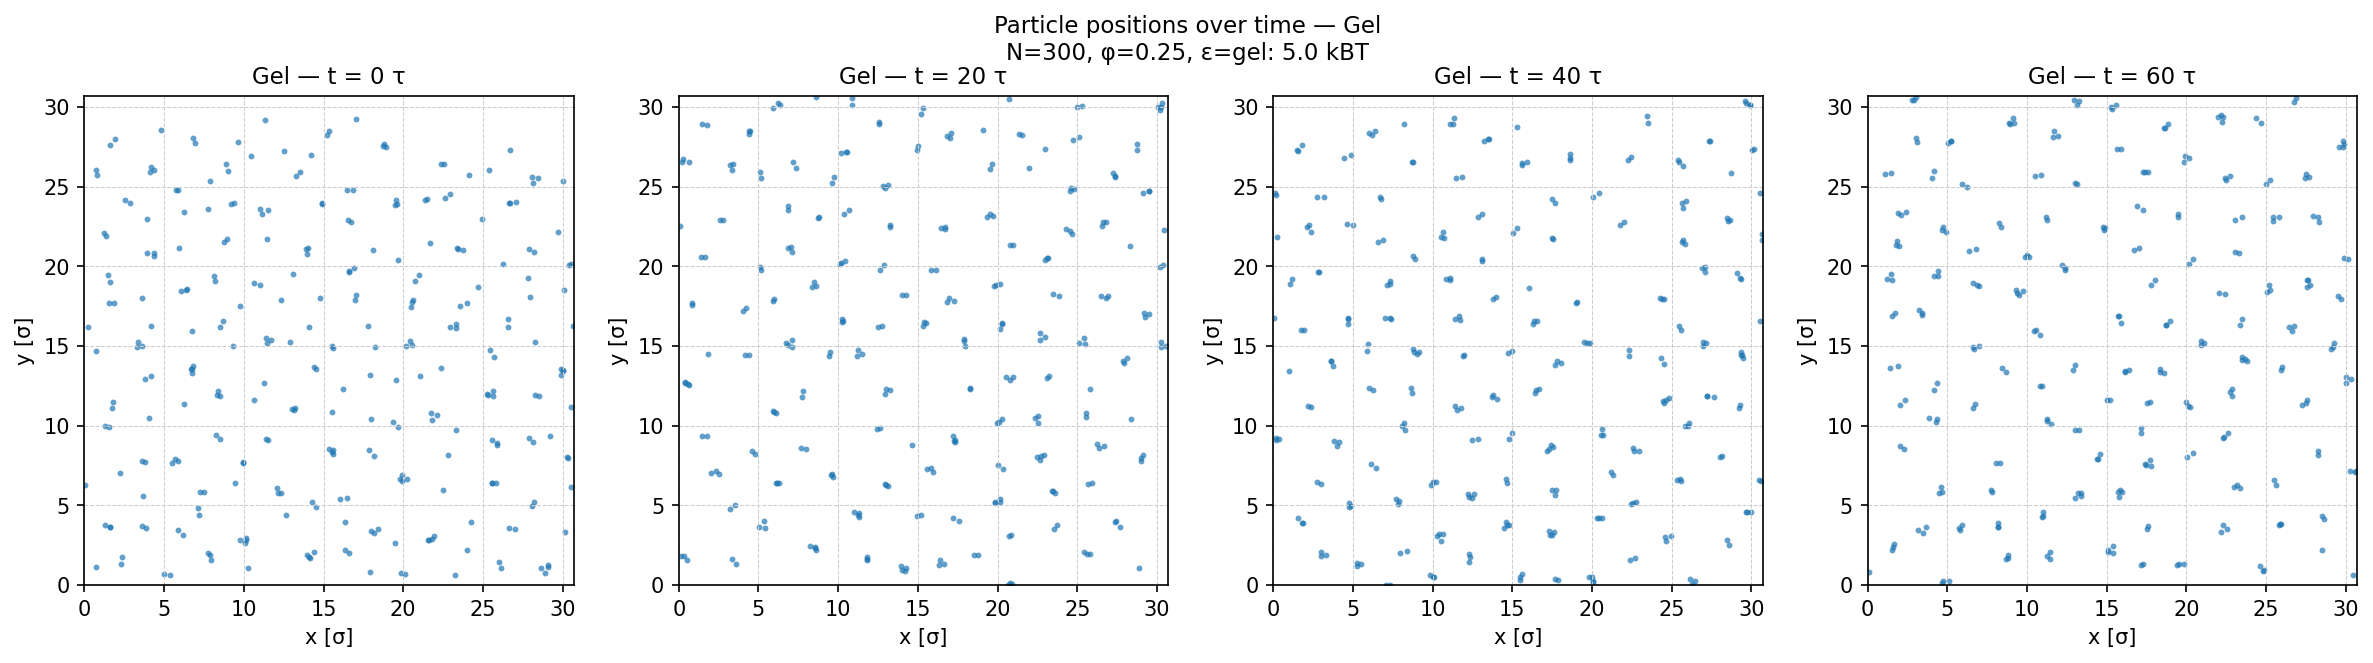
\includegraphics[width=\textwidth]{01_positions_gel.png}
\caption{Particle configurations for the gel ($\varepsilon=5k_BT$) at $t=0$, $20$, $40$ and $60\tau$. Small clusters begin to form, but a fully percolated network is not yet established within this simulation window.}
\label{fig:positions_gel}
\end{figure}

Figure~\ref{fig:positions_liquid} shows the corresponding configurations for the liquid reference, $\varepsilon=1.5k_BT$. While both systems develop clusters, the liquid exhibits faster coarsening and forms larger aggregates within the simulation window. In contrast, the strongly attractive system remains dominated by numerous small clusters, suggesting that particle mobility is reduced before significant domain growth can occur.

\begin{figure}[H]
\centering
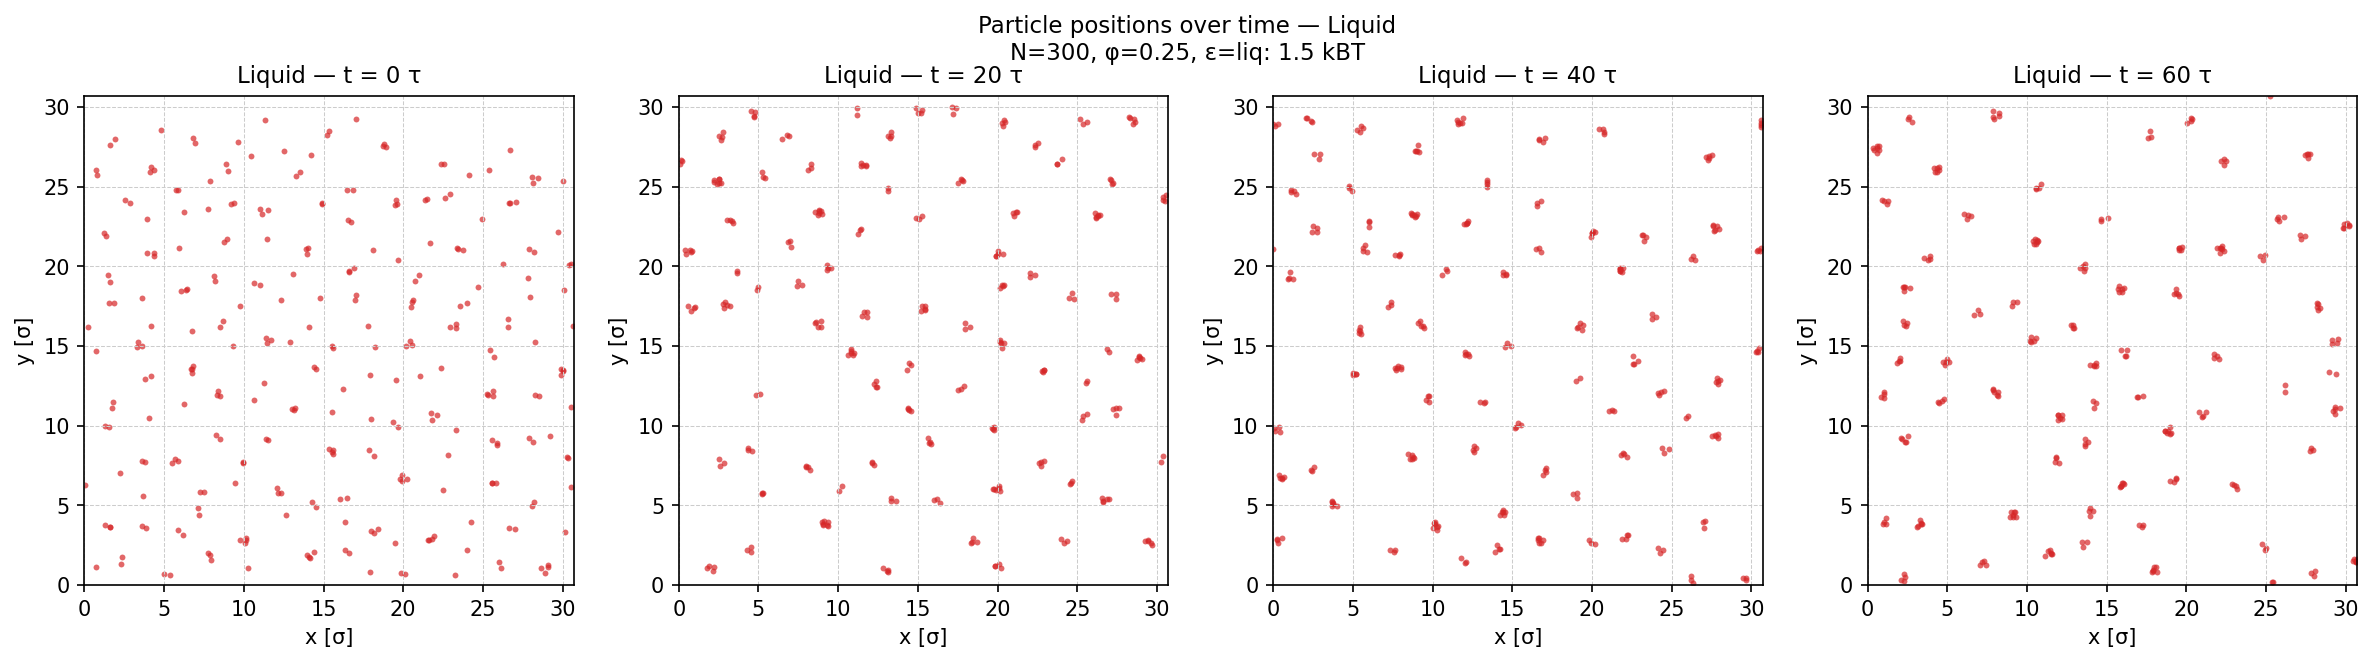
\includegraphics[width=\textwidth]{01_positions_liquid.png}
\caption{Particle configurations for the liquid reference ($\varepsilon=1.5k_BT$) at $t=0$, $20$, $40$ and $60\tau$. Clustering is visible but more transient than in the gel; the system remains spatially more homogeneous throughout the simulation.}
\label{fig:positions_liquid}
\end{figure}

% ============================================================
\section{Results: Structure Factor Analysis}

\subsection{$S(k,t)$ Evolution}

Figure~\ref{fig:sk_gel} shows the time evolution of $S(k,t)$ for the gel. A dominant peak develops around $k^*\simeq 2.5\,\sigma^{-1}$, corresponding to a characteristic domain size $\ell^*=2\pi/k^*\simeq2.5\sigma$, i.e. approximately two to three particle diameters. The peak position shows little systematic drift, which is qualitatively consistent with the onset of arrest: the dominant length scale becomes approximately frozen. The curves remain noisy due to the limited system size.

\begin{figure}[H]
\centering
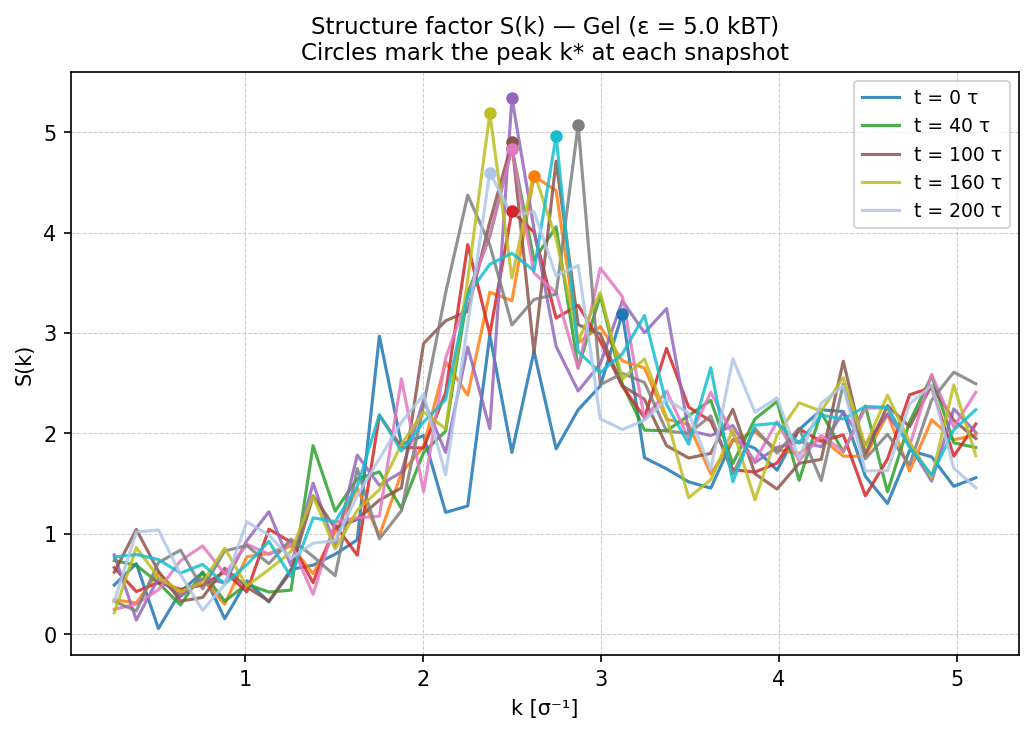
\includegraphics[width=0.88\textwidth]{02_Sk_evolution_gel.png}
\caption{Time evolution of $S(k,t)$ for the gel ($\varepsilon=5k_BT$). A peak forms around $k^*\simeq2.5\,\sigma^{-1}$ and remains approximately stable in position. Circles mark the peak position $k^*$ at each snapshot.}
\label{fig:sk_gel}
\end{figure}

Figure~\ref{fig:sk_liquid} shows $S(k,t)$ for the liquid reference. In contrast to the gel, the peak amplitude grows more strongly and the peak position tends to drift towards lower $k$ values over time, consistent with the growth of the characteristic length scale $\ell(t)=2\pi/k^*(t)$ during coarsening.

\begin{figure}[H]
\centering
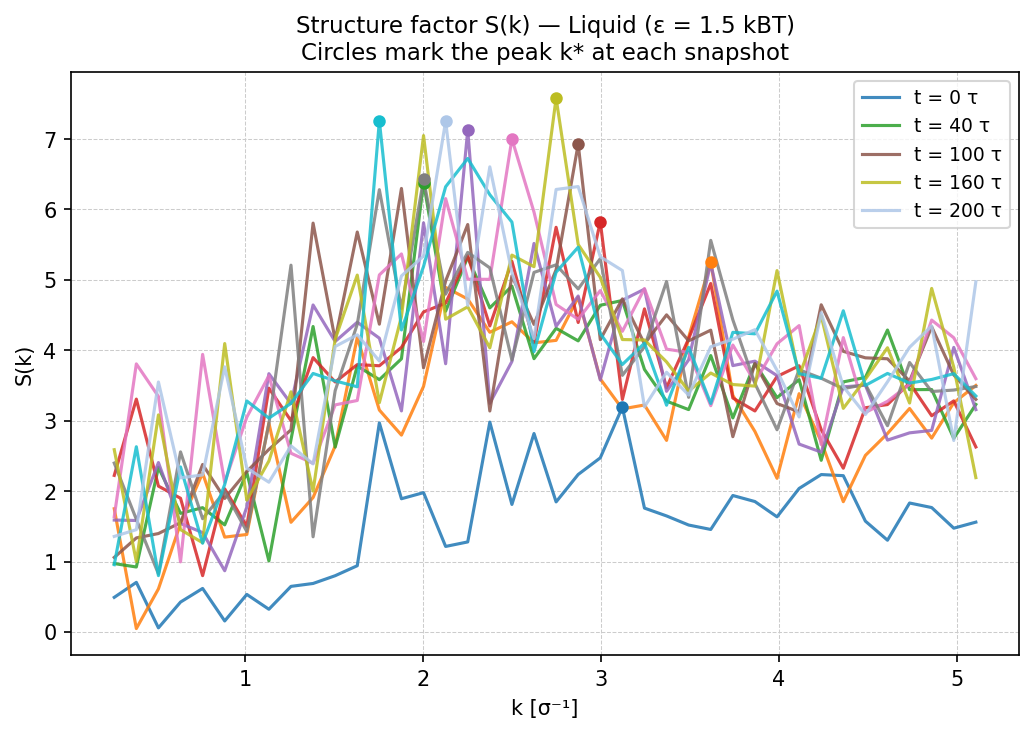
\includegraphics[width=0.88\textwidth]{02_Sk_evolution_liquid.png}
\caption{Time evolution of $S(k,t)$ for the liquid reference ($\varepsilon=1.5k_BT$). The peak amplitude grows and the peak position tends to drift towards lower $k$, consistent with ongoing coarsening without complete arrest.}
\label{fig:sk_liquid}
\end{figure}

\subsection{Final Structure Factor: Gel vs Liquid}

Figure~\ref{fig:sk_final} directly compares the final structure factors at
$t = 200\tau$. The liquid exhibits a sharper and higher peak than the gel.
More importantly, the comparison with the time evolution of $S(k,t)$ shows
that, in the liquid reference, the dominant peak progressively shifts towards
smaller wavevectors. This drift to lower $k$ is the clearest signature of
ongoing coarsening, since it corresponds to an increase of the characteristic
length scale $\ell(t)=2\pi/k^\ast(t)$.

By contrast, in the strongly attractive system, the peak position evolves much
less systematically within the same simulation window. This suggests that
domain growth is strongly slowed down, although the data remain too noisy
to claim a fully arrested gel. The gel regime should therefore be interpreted
as an incipient arrest state: small clusters form and persist, but a fully
percolated frozen network is not yet obtained.

The higher final peak in the liquid is therefore not contradictory. It reflects
the fact that the liquid remains sufficiently mobile to reorganise and coarsen,
whereas the strongly attractive system becomes dynamically hindered before
large-scale density correlations can fully develop.

\begin{figure}[H]
\centering
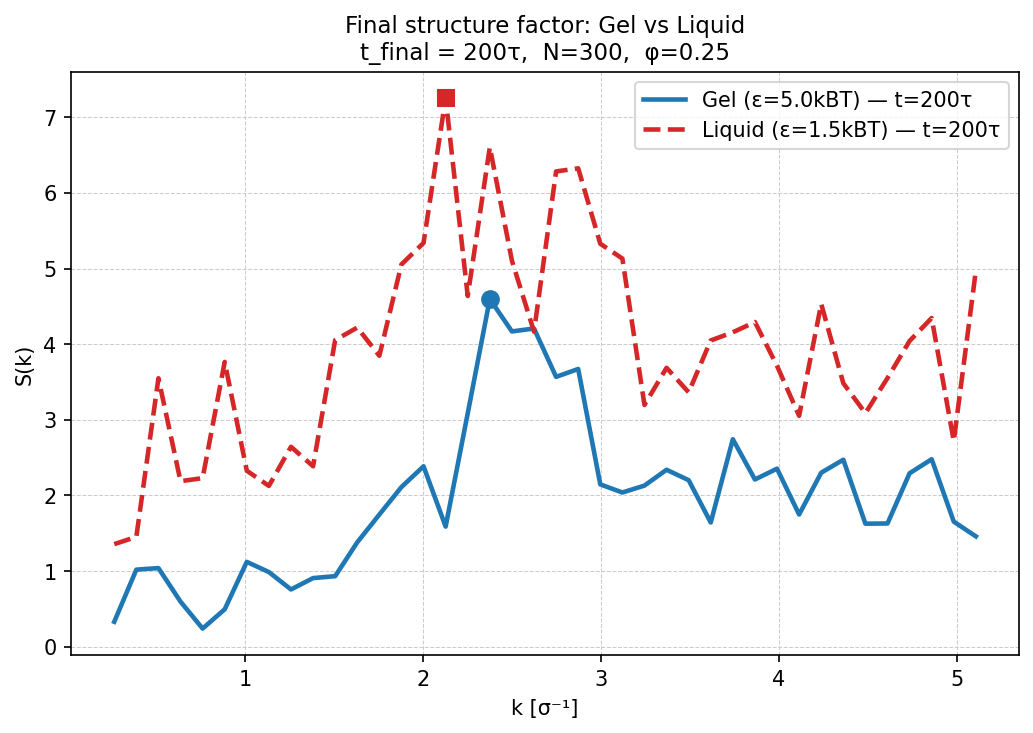
\includegraphics[width=0.82\textwidth]{03_Sk_final_comparison.png}
\caption{Final structure factor $S(k)$ at $t=200\tau$ for the gel and the liquid reference. The liquid has a higher peak amplitude, reflecting continued coarsening. The gel shows a lower but more stable peak consistent with incipient arrest.}
\label{fig:sk_final}
\end{figure}

\subsection{Peak Wavevector $k^*(t)$}

Figure~\ref{fig:kstar} shows the time evolution of the peak wavevector $k^\ast(t)$.
After an initial decrease, the gel remains centred around
$k^\ast \simeq 2.5\,\sigma^{-1}$ and does not exhibit a clear long-term drift
towards smaller wavevectors. This suggests that domain growth is strongly
slowed down compared with the liquid reference. However, significant
fluctuations persist at late times, indicating that the characteristic length
scale is not fully frozen within the simulation window.

The liquid reference exhibits a noisier but overall clearer tendency for
$k^\ast$ to shift towards smaller wavevectors, consistent with continued
coarsening and growth of the characteristic domain size.
\begin{figure}[H]
\centering
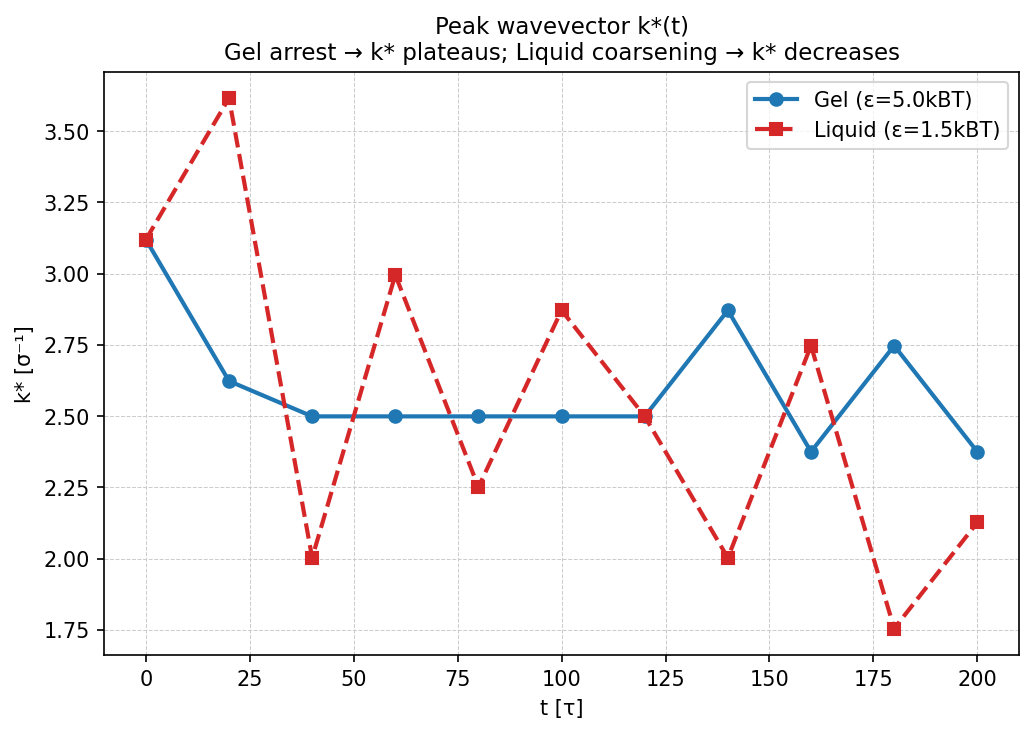
\includegraphics[width=0.78\textwidth]{04_kstar_vs_time.png}
\caption{Peak wavevector $k^*(t)$ as a function of time. The gel plateaus around $k^*\simeq2.5\,\sigma^{-1}$, indicating a nearly frozen characteristic domain size. The liquid tends to shift towards lower $k$, consistent with diffusive coarsening.}
\label{fig:kstar}
\end{figure}

\subsection{Peak Amplitude $S(k^*,t)$}

Figure~\ref{fig:sstar} shows the amplitude of $S(k,t)$ at the peak as a function of time. The liquid reference grows rapidly and reaches a higher value than the gel. The gel grows more slowly and tends to level off around a value of order five. This saturation is consistent with the arrest scenario, although the absence of a fully developed percolated network means that the signal should be interpreted as an early-stage or incipient arrest rather than a complete gel.

\begin{figure}[H]
\centering
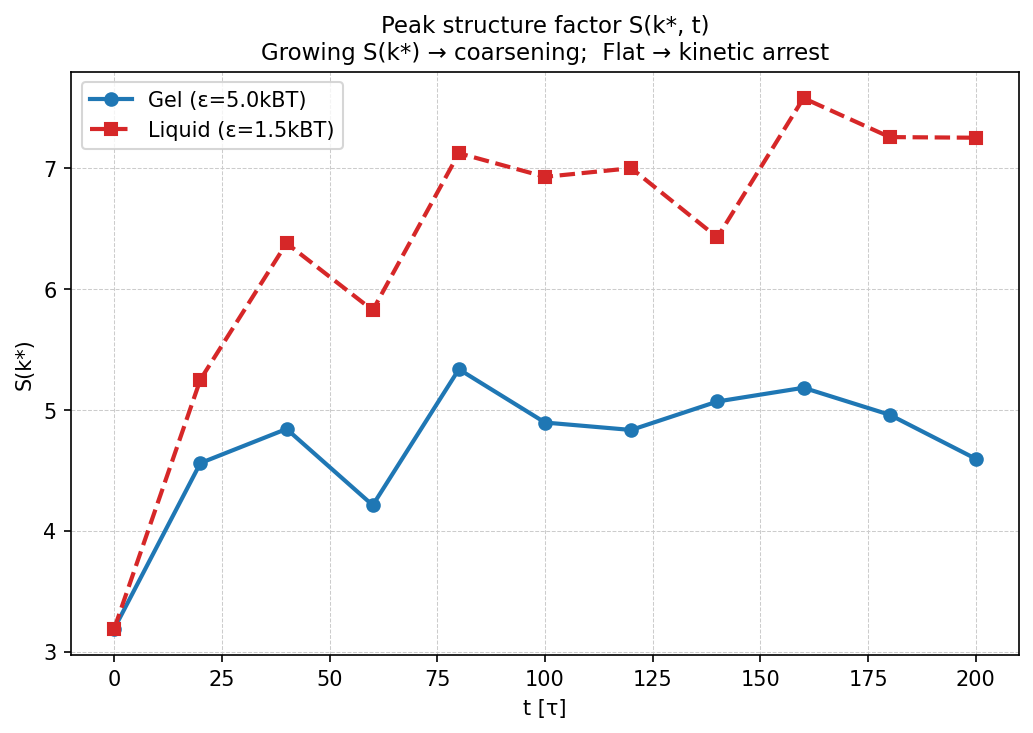
\includegraphics[width=0.78\textwidth]{05_Sstar_vs_time.png}
\caption{Peak structure-factor amplitude $S(k^*,t)$ as a function of time. The liquid grows continuously to larger values, while the gel saturates around a lower value, consistent with the slowing down of structural evolution.}
\label{fig:sstar}
\end{figure}

\subsection{Final Particle Configurations: Gel vs Liquid}

Figure~\ref{fig:final_positions} shows the final particle positions side by side. The gel exhibits small clusters distributed throughout the box, with relatively uniform inter-cluster spacing. The stronger attraction in the gel leads to longer-lived bonds, which hinder cluster rearrangements and slow down the merging of neighbouring aggregates. The liquid shows more compact clusters and a broader distribution of cluster sizes, reflecting more advanced coarsening. Neither system shows a fully percolated network at $t=200\tau$, confirming that longer simulation times or stronger attractions are needed for a complete characterisation of gelation.

\begin{figure}[H]
\centering
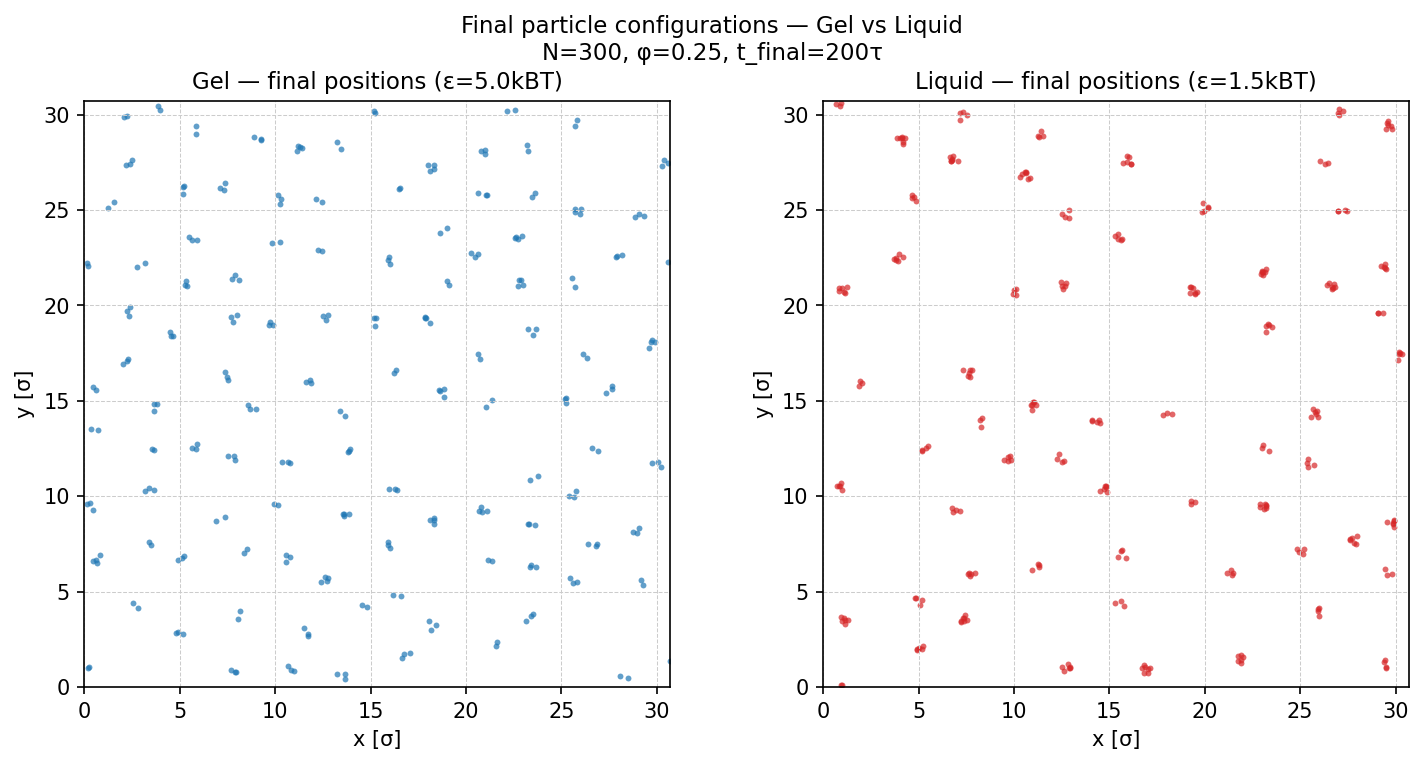
\includegraphics[width=\textwidth]{06_final_positions_comparison.png}
\caption{Final particle configurations at $t=200\tau$ for the gel and the liquid reference. The gel shows small frozen clusters, while the liquid shows more compact clusters due to continued coarsening.}
\label{fig:final_positions}
\end{figure}

% ============================================================
\section{Results: MSD and Ageing Analysis}
\label{sec:msd_ageing}

\subsection{MSD of the Gel}

Figure~\ref{fig:msd_gel} shows the mean-squared displacement of the gel as a function of lag time $\Delta t=t-t_w$ for four waiting times $t_w\in\{0,50,100,150\}\tau$, in both linear and log--log scales. The dashed line indicates free diffusion, $\mathrm{MSD}=4D\Delta t$ in two dimensions.

All curves fall below the free-diffusion line, indicating that attractive interactions slow down particle motion. The log--log plot reveals sub-diffusive behaviour at intermediate lag times, consistent with particles exploring a rough energy landscape created by attractive bonds. However, the expected ageing signature in a fully arrested gel, namely a systematic downward shift of the MSD curves as $t_w$ increases, remains weak here. The curves remain close together, confirming that arrest is not yet complete for $\varepsilon=5k_BT$ within $200\tau$.

\begin{figure}[H]
\centering
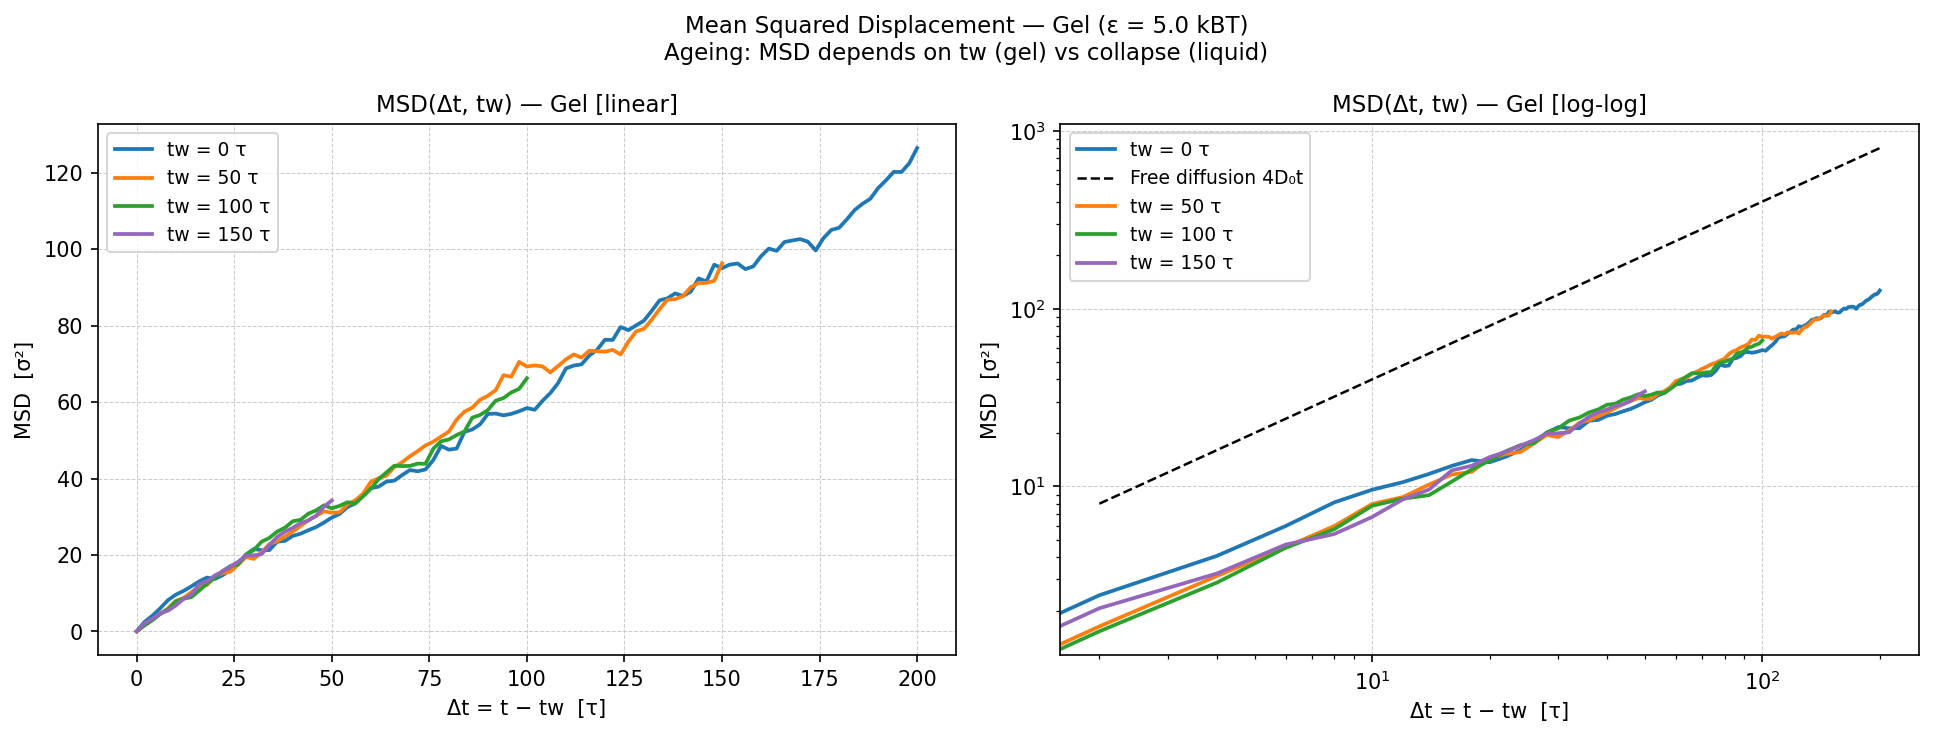
\includegraphics[width=\textwidth]{07_MSD_gel.png}
\caption{MSD$(\Delta t,t_w)$ for the gel ($\varepsilon=5k_BT$) in linear and log--log scales. All curves fall below free diffusion. The spread between $t_w$ curves is marginal, indicating incomplete arrest.}
\label{fig:msd_gel}
\end{figure}

\subsection{MSD of the Liquid Reference}

Figure~\ref{fig:msd_liquid} shows the MSD for the liquid reference. An ergodic liquid should show MSD curves that are approximately independent of $t_w$. This approximate collapse is observed for later waiting times, although the $t_w=0$ curve may reflect an initial transient after the start of the simulation. Compared with the gel, the liquid remains more mobile and does not show a clear cage plateau.

\begin{figure}[H]
\centering
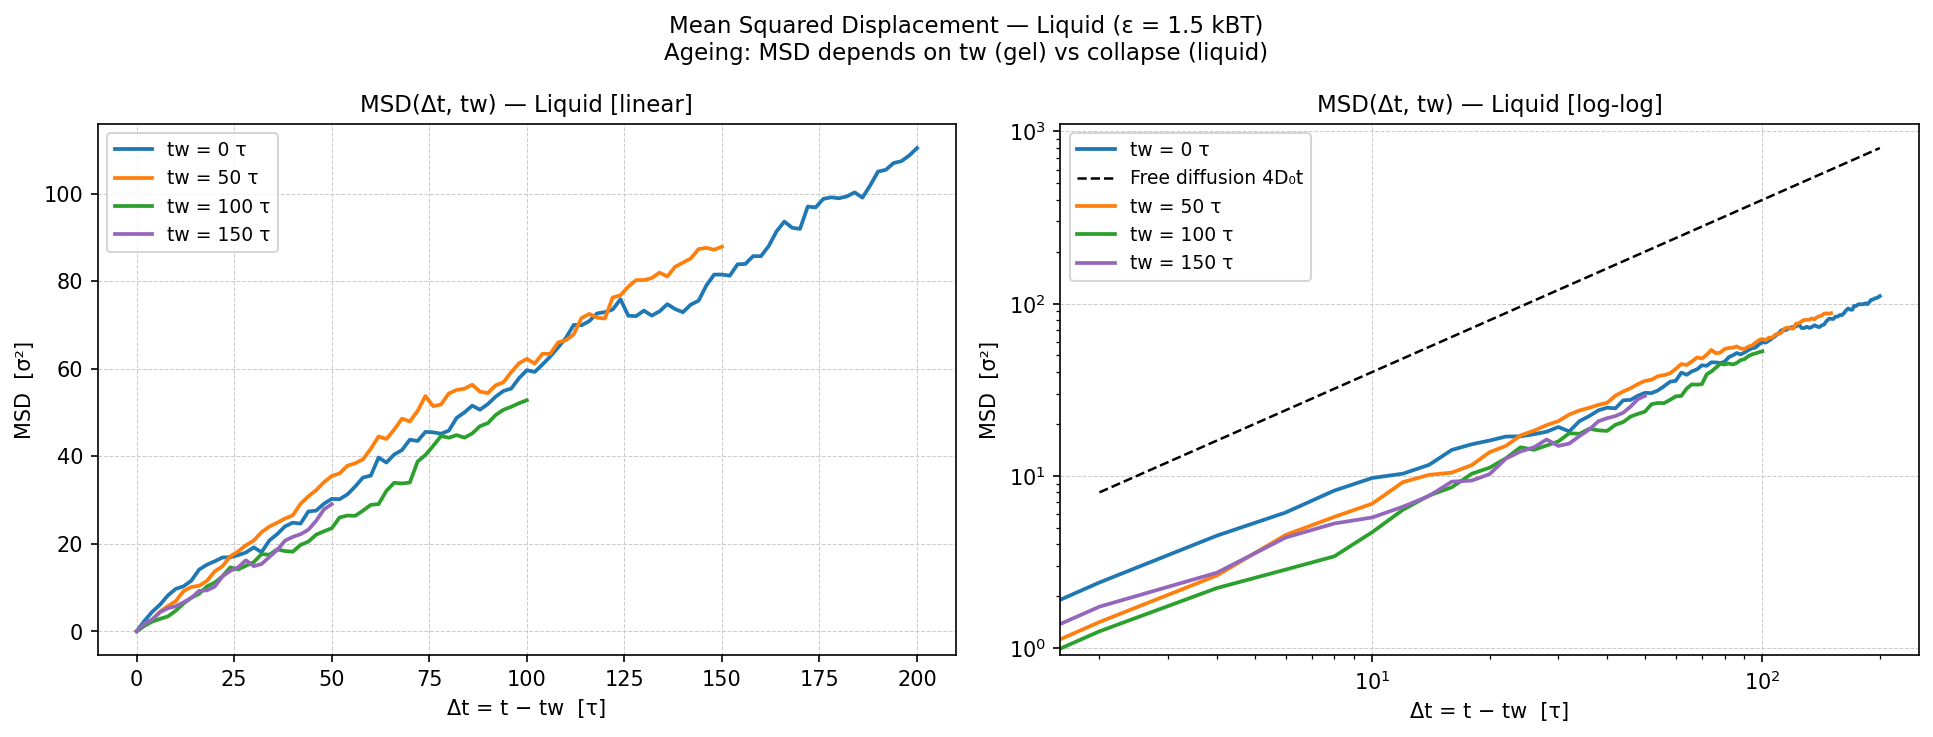
\includegraphics[width=\textwidth]{07_MSD_liquid.png}
\caption{MSD$(\Delta t,t_w)$ for the liquid reference ($\varepsilon=1.5k_BT$) in linear and log--log scales. The approximate collapse of later waiting-time curves is consistent with ergodic behaviour.}
\label{fig:msd_liquid}
\end{figure}

\subsection{Ageing Comparison: Gel vs Liquid}

Figure~\ref{fig:ageing_comparison} directly compares the gel and liquid MSD in log--log scale for all four waiting times. In a fully arrested gel, the gel panel should show clearly separated curves, with larger $t_w$ corresponding to lower MSD values. The liquid panel should show collapsed curves. In the present results, both panels show qualitatively similar behaviour, with only a modest spread between waiting times. The gel panel shows slightly less collapse than the liquid panel, which is physically consistent with incipient non-ergodicity, but it is not yet a conclusive ageing signature.

\begin{figure}[H]
\centering
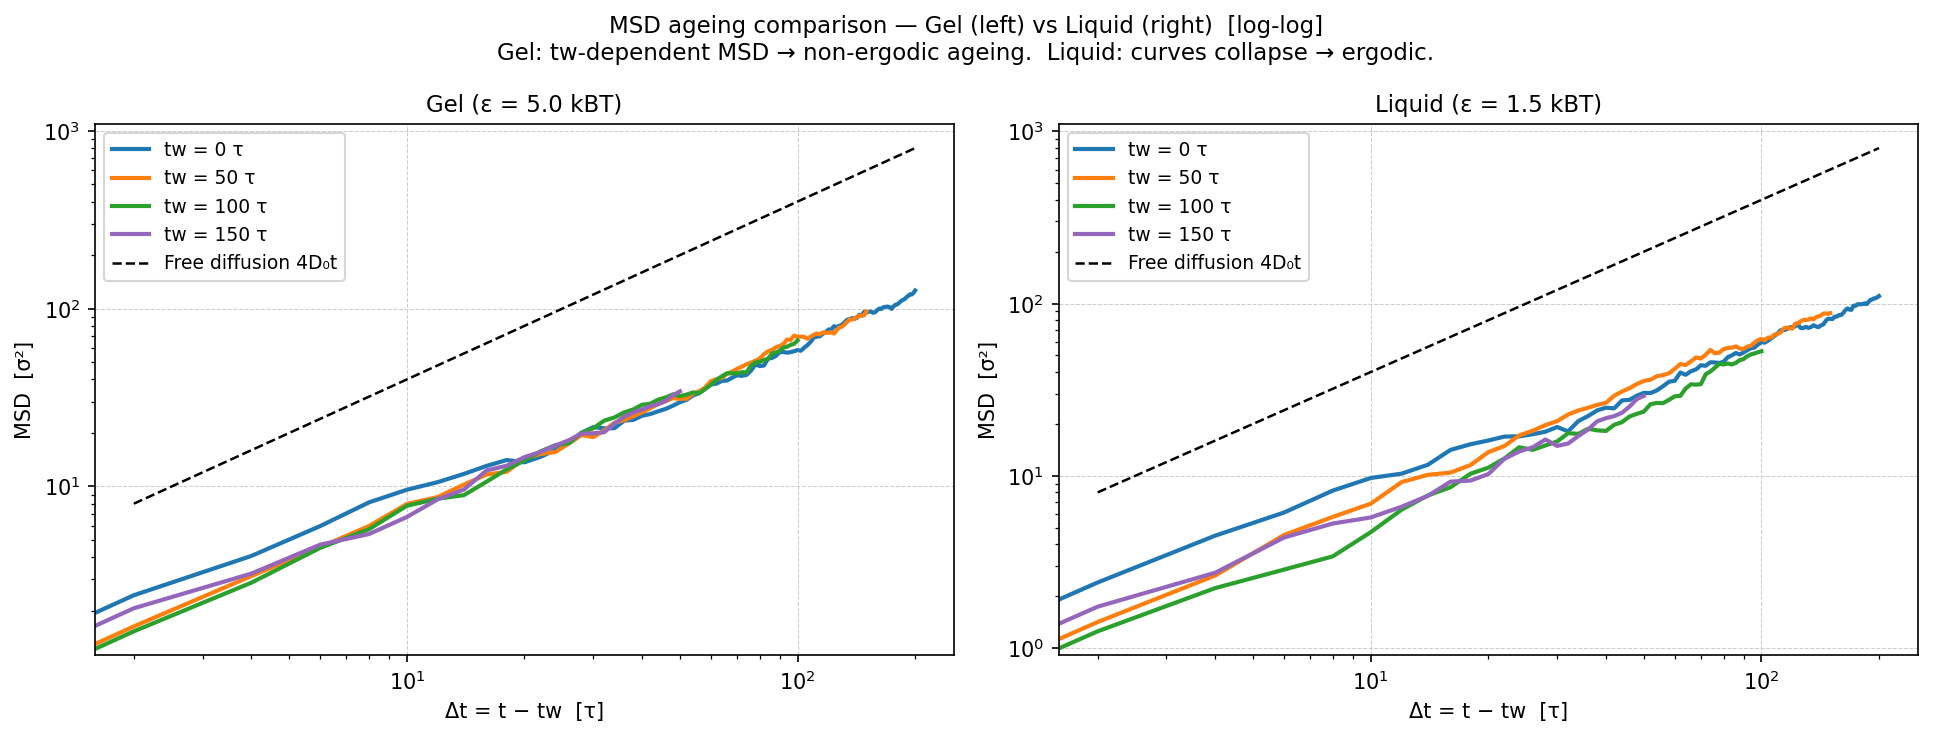
\includegraphics[width=\textwidth]{08_MSD_ageing_comparison.png}
\caption{MSD ageing comparison in log--log scale: gel versus liquid reference. The gel shows slightly less collapse than the liquid, consistent with incipient non-ergodicity, but a conclusive ageing signal requires longer simulations or stronger attractions.}
\label{fig:ageing_comparison}
\end{figure}

Figure~\ref{fig:msd_tw} shows the MSD at a fixed lag time $\Delta t\simeq20\tau$ as a function of waiting time. In an ageing gel, this quantity is expected to decrease with $t_w$. In the present simulation, the gel curve is nearly flat, whereas the liquid curve decreases more strongly, indicating that this observable is not yet a robust ageing marker for the current data set. The result reinforces the conclusion that the gel is only partially arrested.

\begin{figure}[H]
\centering
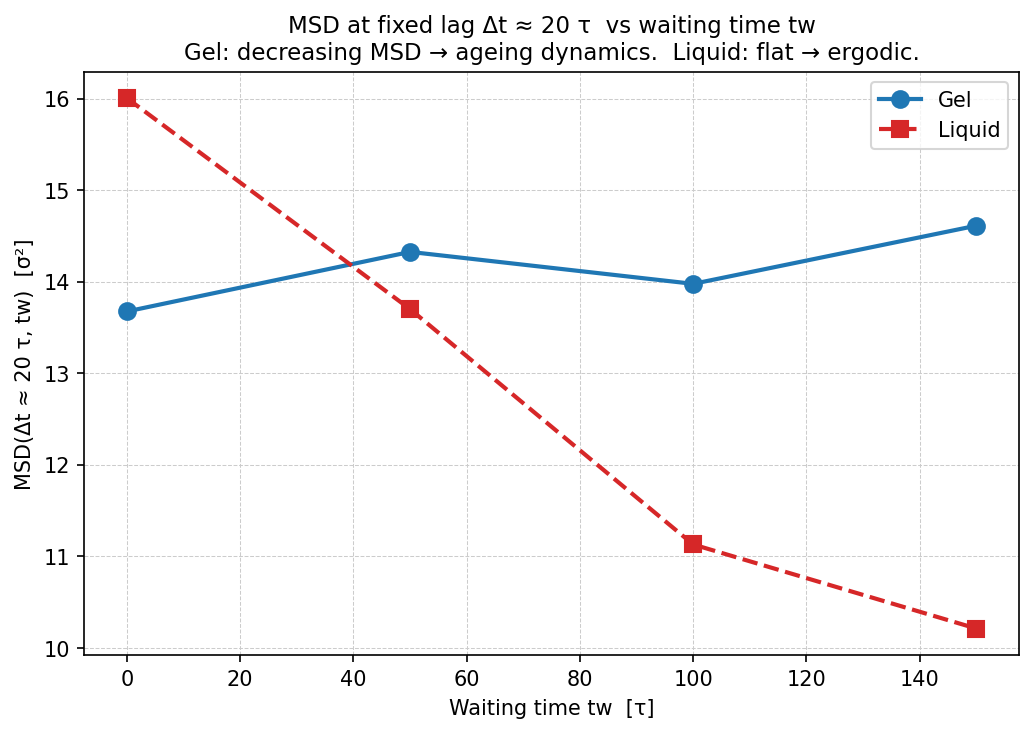
\includegraphics[width=0.78\textwidth]{09_MSD_vs_tw.png}
\caption{MSD at fixed lag time $\Delta t\simeq20\tau$ as a function of waiting time $t_w$. A clear decrease in the gel would indicate ageing, but the present data show only a weak or ambiguous signal.}
\label{fig:msd_tw}
\end{figure}

% ============================================================
\section{Limitations and Perspectives}

The present results are obtained with $N=300$ particles and $t_{\mathrm{final}}=200\tau$. Several limitations should be noted.

First, the finite system size limits the accessible range of wavevectors. With a finite box, the smallest available wavevector is of order $2\pi/L$, which restricts the observation of very large-scale density fluctuations. This contributes to the noise in $S(k,t)$ and makes the extraction of $k^*(t)$ sensitive to finite-size effects.

Second, the simulation time remains too short to observe a fully arrested colloidal gel. The MSD continues to grow over the accessible time window and does not display a clear cage plateau. This indicates that particles remain mobile and that the network is not yet fully frozen. Longer simulations, or a larger attraction strength such as $\varepsilon=8k_BT$, should produce stronger arrest and clearer ageing signatures.

Third, ageing statistics remain limited because only four waiting times are considered. A more systematic ageing analysis would require more values of $t_w$, longer trajectories, and ensemble averaging over several independent runs.

Finally, the simulation is two-dimensional. Gelation thresholds, percolation properties, and scaling exponents differ from those of three-dimensional experimental systems. Therefore, the present simulation should be interpreted as a minimal numerical model rather than a quantitatively faithful model of a specific experimental gel.

% ============================================================
\section{Conclusion}

This work presented a theoretical and numerical framework for studying colloidal gelation as arrested phase separation. A minimal Brownian Dynamics model of attractive particles was implemented and analysed using the structure factor and the mean-squared displacement.

Several numerical corrections were required: the time step was reduced to stabilise the integration, the simulation time was extended to $200\tau$, and the original purely repulsive reference state was replaced by a weakly attractive liquid reference. An ageing protocol was implemented by tracking unwrapped particle trajectories and computing the MSD for multiple waiting times.

The simulation results show qualitative differences between the strongly attractive and weakly attractive regimes. The liquid reference exhibits stronger peak growth and a clearer tendency for $k^\ast(t)$ to shift towards smaller wavevectors, consistent with ongoing coarsening and the growth of larger domains. In contrast, the evolution of the peak position in the strongly attractive system is weaker and less systematic, suggesting a slowing down of domain growth without complete kinetic arrest within the simulation window. The MSD curves of the gel lie below the free-diffusion line, indicating slowed-down dynamics due to attractive bonding.

However, the gel is not yet fully arrested within $200\tau$ at $\varepsilon=5k_BT$. The MSD does not show a clear cage plateau and the waiting-time dependence remains marginal. The present results should therefore be described as early-stage clustering or incipient kinetic arrest rather than a fully developed colloidal gel. Future simulations with stronger attraction, longer times, larger system sizes, and better ensemble averaging are expected to produce a clearer arrested network, stronger MSD plateaus, and a more conclusive ageing signature.

% ============================================================
\begin{thebibliography}{9}

\bibitem{doi_edwards}
M. Doi and S. F. Edwards,
\textit{The Theory of Polymer Dynamics},
Oxford University Press, 1996.

\bibitem{doi_soft}
M. Doi,
\textit{Soft Matter Physics},
Oxford University Press, 2013.

\bibitem{trappe}
V. Trappe, V. Prasad, L. Cipelletti, P. N. Segre and D. A. Weitz,
``Jamming phase diagram for attractive particles'',
\textit{Nature} \textbf{411}, 772--775 (2001).

\bibitem{lu}
P. J. Lu, E. Zaccarelli, F. Ciulla, A. B. Schofield, F. Sciortino and D. A. Weitz,
``Gelation of particles with short-range attraction'',
\textit{Nature} \textbf{453}, 499--503 (2008).

\bibitem{israelachvili}
J. N. Israelachvili,
\textit{Intermolecular and Surface Forces}, 3rd ed.,
Academic Press, 2011.

\bibitem{foffi}
G. Foffi, C. De Michele, F. Sciortino and P. Tartaglia,
``Evidence for an unusual dynamical-arrest scenario in short-ranged colloidal systems'',
\textit{Physical Review E} \textbf{65}, 050802(R) (2002).

\bibitem{kloeden}
P. E. Kloeden and E. Platen,
\textit{Numerical Solution of Stochastic Differential Equations},
Springer, 1992.

\end{thebibliography}

\end{document}
